% \chapter*{Templates}

% \begin{figure}[htb]
% \centering
% \begin{tikzpicture}
%   \begin{axis}[
%     width=\textwidth,
%     height=9.5cm,
%     ybar=0pt, % Raum zwischen den Balken
%     bar width=40pt,
%     enlarge x limits=0.5,
%     legend style={at={(1,1.15)},anchor=north east,draw=none},% Legende über Abb.
%     legend cell align=left,% Linksbündige Ausrichtung der Legende
%     % xlabel={Gesicht},
%     xtick={data},
%     symbolic x coords={hoch vertrauenswürdig,niedrig vertrauenswürdig},
%     ymin=17,
%     ymax=25,
%     ylabel={Mittlerer Einsatz},
%     %ytick={17,18,...,25}
%   ]
%     \addplot[
%         black,fill=lightgray
%       ]coordinates {
%       (hoch vertrauenswürdig,23.453) 
%       (niedrig vertrauenswürdig,18.797)
%     };
%     % \addlegendentry{~betrügerisches Verhalten};
%     % \addplot[
%     %     black,fill=white,
%     %     postaction={pattern=north east lines,pattern color=gray}
%     %     ] coordinates {
%     %   (hoch vertrauenswürdig,22.891) +- (0,0.410)
%     %   (niedrig vertrauenswürdig,18.844) +- (0,0.407)
%     % };
%     % \addlegendentry{~kooperatives Verhalten};
%   \end{axis}
% \end{tikzpicture}
% \caption{Investitionsverhalten. Die Fehlerbalken stellen die Standardfehler dar.}
% \label{fig:Investitionsverhalten}
% \end{figure}

% \begin{figure}[H]
% 	\centering 
% 	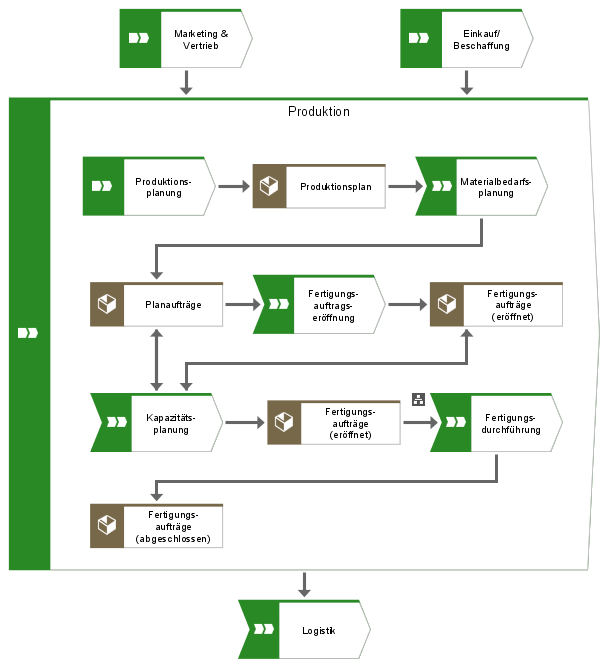
\includegraphics[width=\textwidth]{img/Production_IST.png}	\caption[TEST]{\label{fig:logo}test
% 	}
% \end{figure}


% % \begin{figure}[H]
% % 	\centering 
% % 	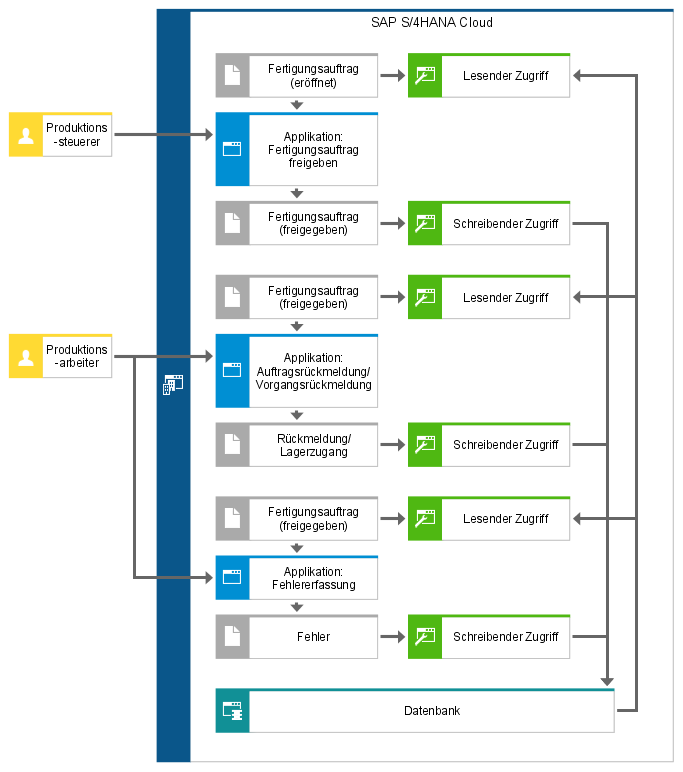
\includegraphics[width=\textwidth]{img/Arch_IST.png}	\caption[TEST]{\label{fig:logo}test
% % 	}
% % \end{figure}

% % \begin{figure}[H]
% % 	\centering 
% % 	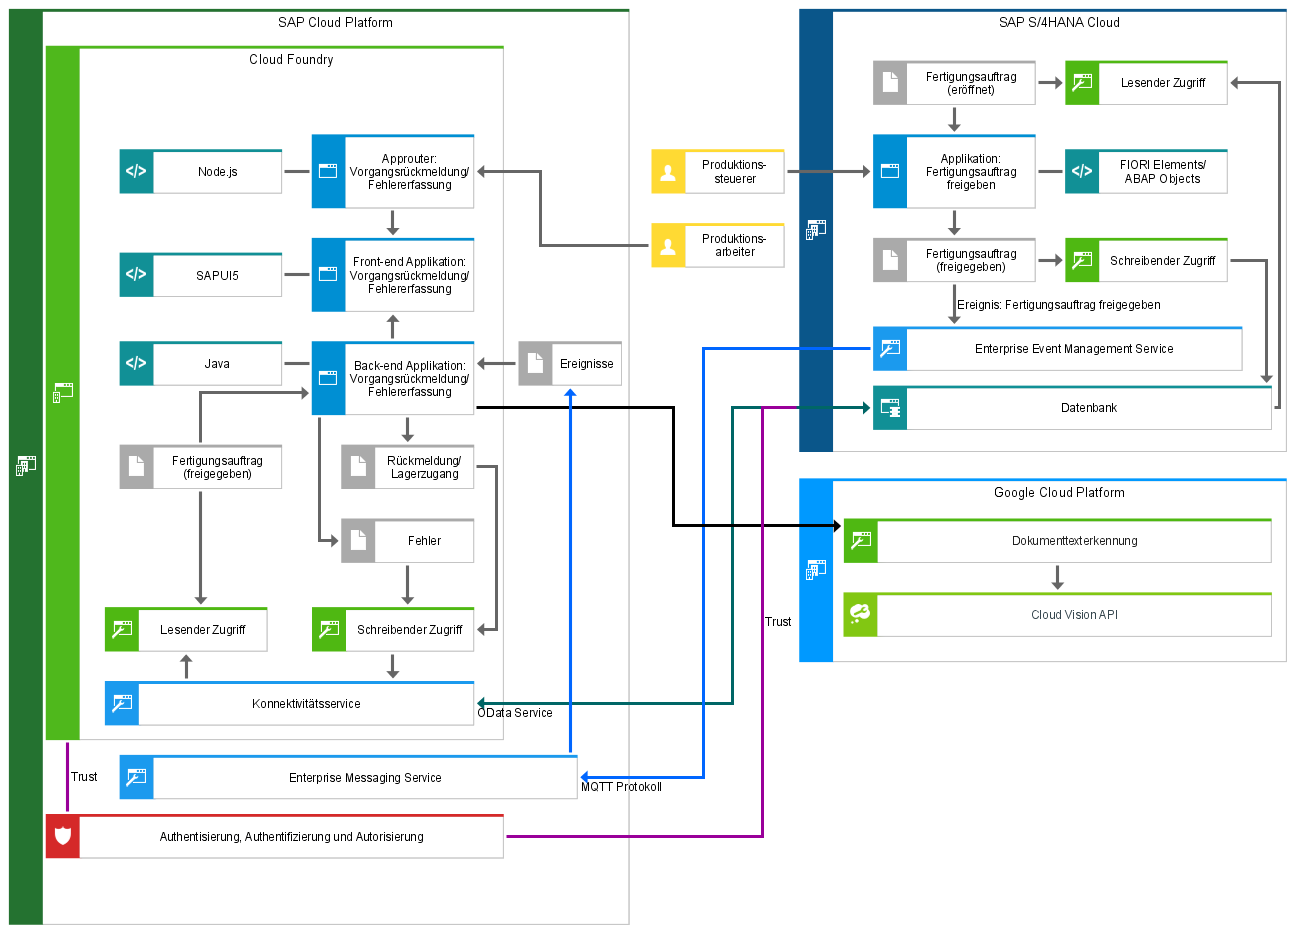
\includegraphics[angle=270,width=\textwidth]{img/Arch_SOLL.png}	\caption[TEST]{\label{fig:logo}test
% % 	}
% % \end{figure}

% % \begin{figure}[H]
% % 	\centering 
% % 	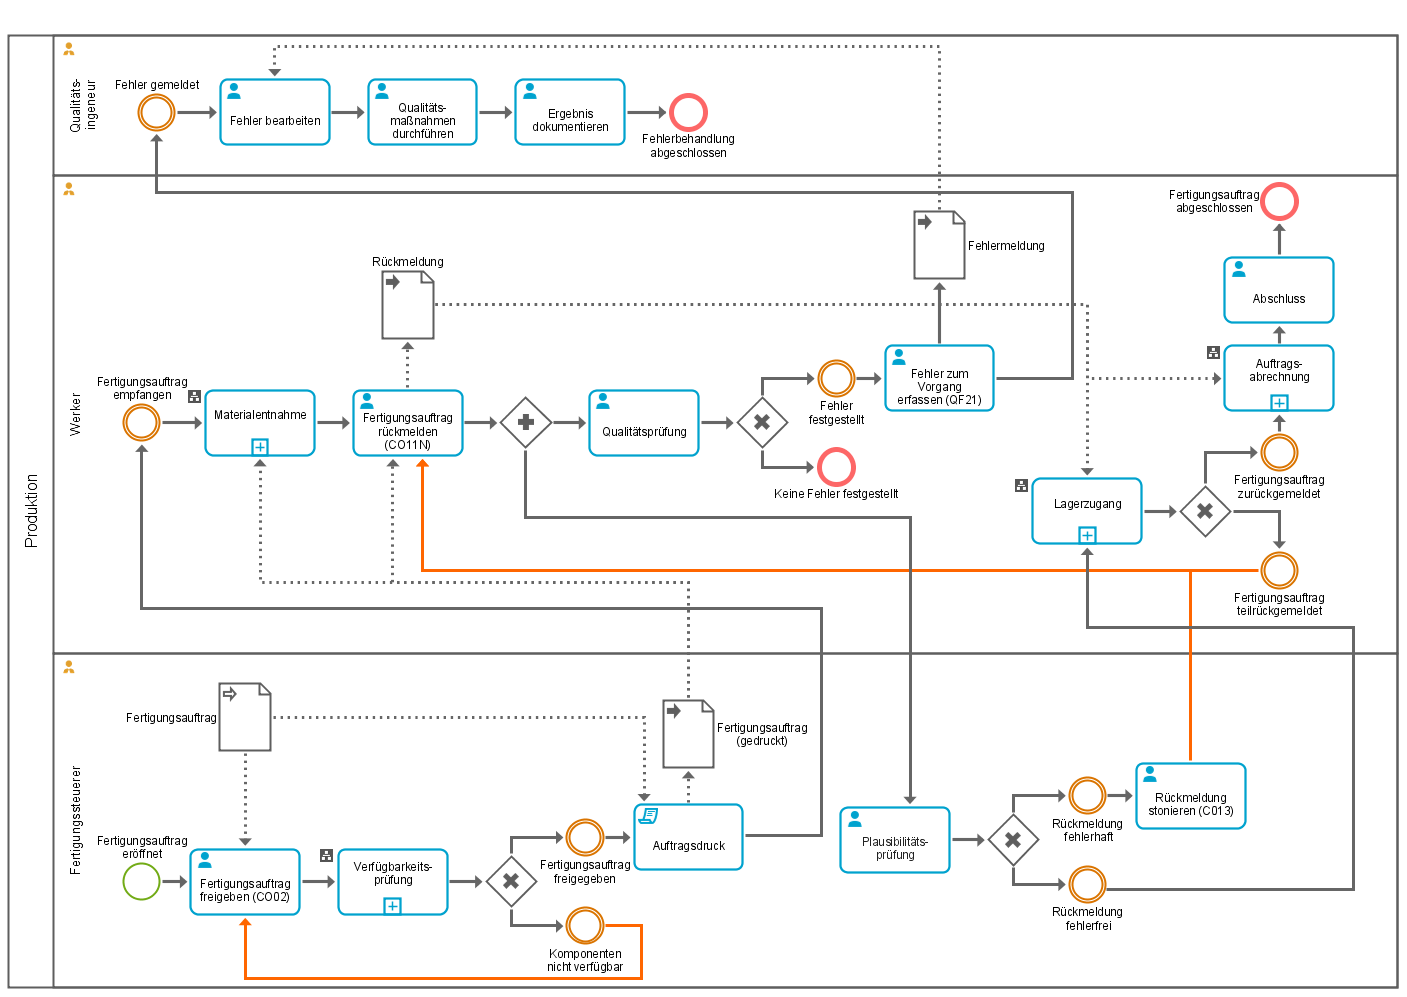
\includegraphics[angle=270,width=\textwidth]{img/Order_Operating_IST.png}	\caption[TEST]{\label{fig:logo}test
% % 	}
% % \end{figure}

% % \begin{figure}[H]
% % 	\centering 
% % 	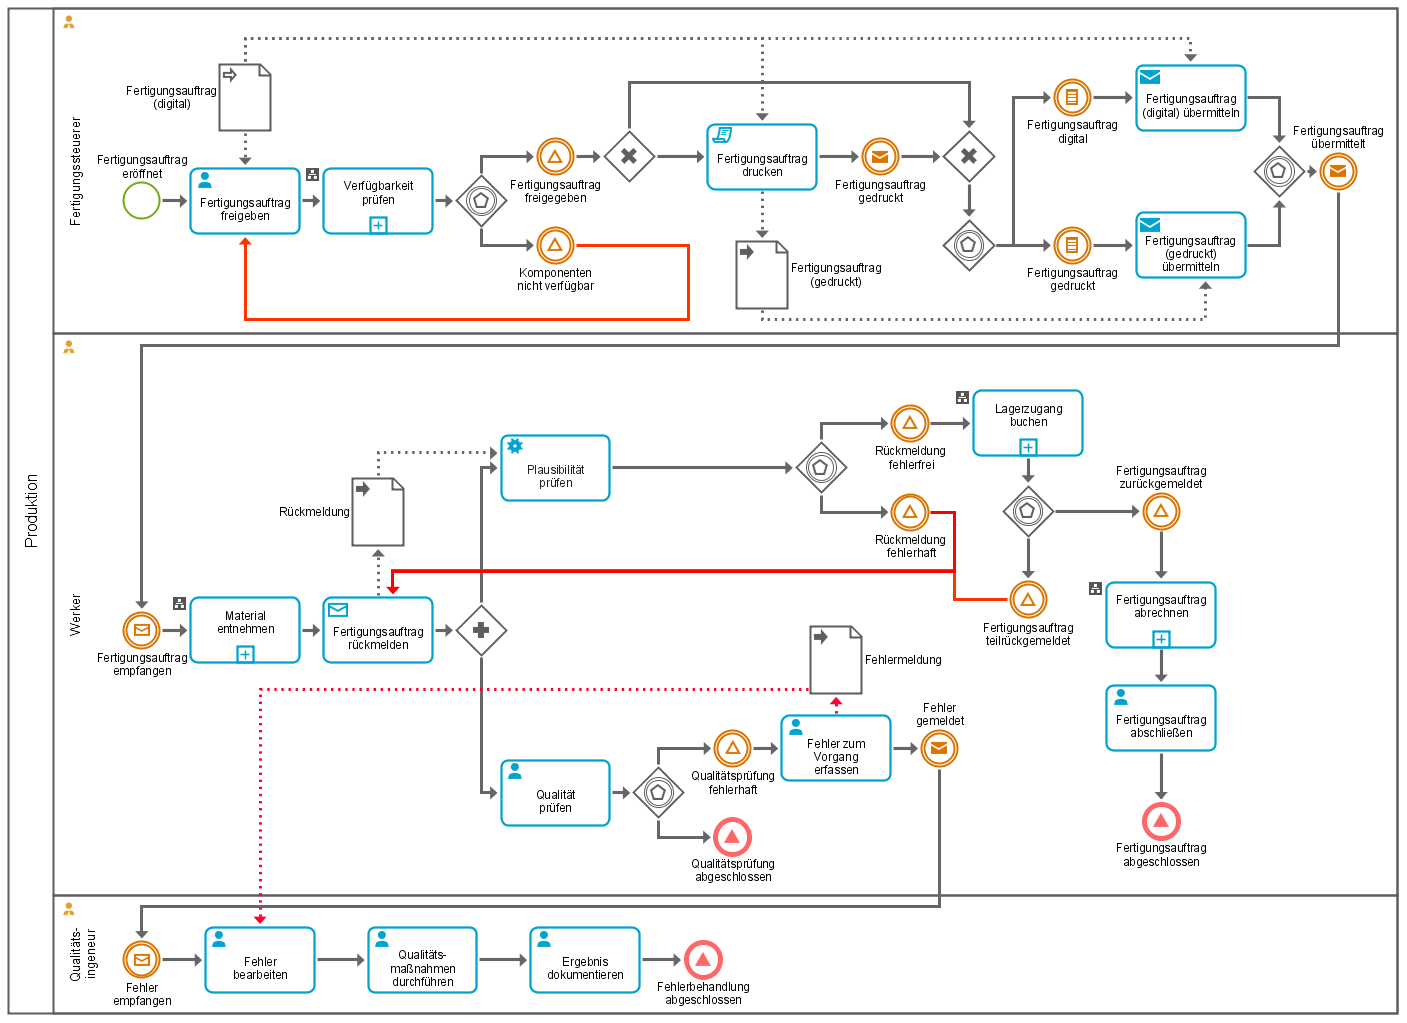
\includegraphics[angle=270,width=\textwidth]{img/Order_Operating_SOLL.png}	\caption[TEST]{\label{fig:logo}test
% % 	}
% % \end{figure}

% % \begin{algorithm}[H]
% % \centering 
% % \inputminted[linenos]{java}{code/Application.java}
% % \caption{Application.java}
% % \end{algorithm}

% % \begin{algorithm}[H]
% % \centering 
% % \inputminted[linenos]{java}{code/MessageController.java}
% % \caption{MessageController.java}
% % \end{algorithm}

% % \begin{algorithm}[H]
% % \centering 
% % \inputminted[linenos]{java}{code/ProductionOrderController.java}
% % \caption{ProductionOrderController.java}
% % \end{algorithm}

% % \begin{algorithm}[H]
% % \centering 
% % \inputminted[linenos]{java}{code/ProductionOrderReleasedNotificationListener.java}
% % \caption{ProductionOrderReleasedNotificationListener.java}
% % \end{algorithm}

% % \begin{algorithm}[H]
% % \centering 
% % \inputminted[linenos]{java}{code/EventMessagingService.java}
% % \caption{EventMessagingService.java}
% % \end{algorithm}

% \begin{algorithm}[H]
% \centering 
% % \lstinputlisting[style=JavaStyle, caption=pr.java]{code/test.java}
% \inputminted[linenos]{js}{code/test.js}
% \caption{test.js}
% \end{algorithm}

% % \begin{algorithm}[H]
% % \centering 
% % % \lstinputlisting[language=ABAP, caption=test.abap]{code/test.abap}
% % \inputminted[linenos]{ABAP}{code/RaiseEvent.abap}
% % \caption{Exemplarisches Auslösen eines Ereignisses in SAP S/4HANA}
% % \end{algorithm}

% % \begin{algorithm}[H]
% % \centering 
% % % \lstinputlisting[language=ABAP, caption=test.abap]{code/test.abap}
% % \inputminted[linenos]{js}{code/test.json}
% % \caption{Exemplarisches Auslösen eines Ereignisses in SAP S/4HANA}
% % \end{algorithm}

% \begin{definitionForm}[Definition]
% Diese Hervorhebungen können für deine Arbeit an machen stellen sehr nützlich sein. Besonders bei Definitionen macht es einen guten Eindruck, wenn diese in solch einer Form dargestellt ist. 
% \end{definitionForm}

% DHBW Richtlinie: Laut den aktuellen Angaben der DHBW sind diese Boxen nicht notwendig. Helfen können sie jedoch, um einen Faktor speziell hervorzuheben. Bitte beachte, dass deine Projektarbeit oder auch Bachelorarbeit kein Bilderbuch ist! Alles was eingebunden wird sollte schlicht und dezent dargestellt sein.

% \begin{attentionForm}[SOA und Webservices sind nicht grundsätzlich synonym]
% An dieser Stelle sei jedoch der Hinweis erlaubt, dass das Konzept der Serviceorientierung allgemeiner ist und schon früher existierte als Webservices. Webservices sollten daher nur als eine, wenn auch zum Verfassungszeitpunkt dieses Buches als wahrscheinlich am besten geeignete Möglichkeit zur Realisierung serviceorientierter Architekturen betrachtet werden.
% \end{attentionForm}



% \begin{table}[H]
% 	\centering
% 	\begin{tabularx}{\textwidth}{|l|X|} 
% 		\hline
% 		Auslöser                                     &   
% 		Der Produktionsplaner möchte Engpässe an betroffenen Arbeitsplätzen durch Modifikationen an Kapazitätsangeboten beheben. \\ 
% 		\hline\hline
% 		Input                                         &   
% 		Handlungsbedarf durch die Auswertung der Kapazitätsauslastung \\ 
% 		\hline\hline
% 		Aktivitäten &   
% 		\begin{minipage}{5in}
%     		\begin{enumerate} 
%         		\renewcommand{\labelenumi}{(\arabic{enumi})}
%         		\item Starten der Anwendung
%         		\item Iterative Vorgehensweise bis zur Zielerreichung:
%             		\begin{enumerate} 
%             		\renewcommand{\labelenumi}{(\arabic{enumi})}
%             		\item Wahl einer Arbeitsplatzkapazität
%             		\item Erstellung einer Angebotskapazität
%             		\item Festlegung eines Gültigkeitszeitraums
%             		\item Pflege von Schichten in der Angebotskapazität
%             		\item Speichern der Änderungen
%             		\end{enumerate}
%             	\item Ende des Prozesses
%     		\end{enumerate}
%     		\vspace{1pt}		
% 		\end{minipage} \\
% 		\hline\hline
% 		Output                                        &   
% 		Modifizierte Kapazitätsangebote von Arbeitsplätzen  \\
% 		\hline
% 	\end{tabularx}
% 	\caption{\label{tab:aktivitäten}Ist-Prozessbeschreibung }
% \end{table}

% \begin{table}[H]
% 	\centering
% 	\begin{tabularx}{\textwidth}{l X} 
% 		\toprule
% 		\textbf{Kriterium}  &   
% 		\textbf{Beschreibung}  \\ 
% 		\midrule
% 		OP1 &   
% 		Keine Modifikationsmöglichkeiten  \\  \cmidrule(r){1-1} \cmidrule(r){2-2}
% 		OP2 &   
% 		Unausgereifter Prozessablauf \\ \cmidrule(r){1-1} \cmidrule(r){2-2}
% 		OP3 &   
% 		Mangelhafte Bedienbarkeit  \\ \cmidrule(r){1-1} \cmidrule(r){2-2}
% 		OP4 &   
% 		Kontraintuitives Stammdatenmodell  \\ \cmidrule(r){1-1} \cmidrule(r){2-2}
% 		OP5 &   
% 		Keine Überprüfung der Validität der Eingaben  \\ \cmidrule(r){1-1} \cmidrule(r){2-2}
% 		OP6 &   
% 		Kein Überblick über getätigte Modifikationen  \\
% 	    \bottomrule
% 	\end{tabularx}
% 	\caption{\label{tab:potentiale}Optimierungspotenziale des Ist-Systems}
% \end{table}



% % \resizebox{\textwidth}{!}{%
% % \begin{tikzpicture}

% % % Fragestellungs
% % \node (goal) [goal] {Entwicklung eines dynamischen Gesch{\"a}ftsprozesses zur ereignisgesteuerten Betriebsdatenerfassung mit SAP S/4HANA Cloud};

% % % Wozu?
% % \node (wozu) [question, node distance=7cm and 0.5cm, above left=of goal] {Wohin?};
% % \draw [] (goal) |- (wozu);


% % % Einleitung
% % \node (einleitung)[main,draw,rectangle, minimum height = 6cm, node distance=0.5cm and 0.5cm, below=of wozu] {};

% % \node (Einleitung) at (einleitung.north) [anchor=north] {\ref{ch:einleitung} \nameref{ch:einleitung}};
% % \node (Motivation) [submain,below=of Einleitung] {Motivation}
% % \node (Problemstellung) [submain, below=of Motivation] {Problemstellung};
% % \node (Zielsetzung) [submain, below=of Problemstellung] {Zielsetzung};
% % \node (Vorgehen) [submain, below=of Zielsetzung] {Vorgehen};

% % \draw [->] (Motivation) -- (Motivation |- Problemstellung.north); 
% % \draw [->] (Problemstellung) -- (Problemstellung |- Zielsetzung.north); 
% % \draw [->] (Zielsetzung) -- (Zielsetzung |- Vorgehen.north); 
% % % \draw [->] (gui1) -- (gui1 |- pssub1.north); 

% % % Was?
% % \node (was) [question, node distance=6cm and 0.5cm, above right=of goal] {Was?};
% % \draw [] (goal) |- (was);

% % % Grundlagen
% % \node (grundlagen)[main,draw,rectangle, minimum height = 4cm, node distance=0.5cm and 0.5cm, below=of was] {};

% % \node (Grundlagen) at (grundlagen.north) [anchor=north] {\ref{ch:Grundlagen} Stand der Wissenschaft und Technik};
% % \node (Automatisierung) [submain,below=of Grundlagen] {Automatisierung von Gesch{\"a}ftsprozessen};
% % \node (pssub2) [submain, below=of Automatisierung] {};

% % \end{tikzpicture}
% % }%
